\chapter{Конструкторский раздел}
В данном разделе приведены схемы алгоритмов умножения матриц, проведены оценки трудоемкости алгоритмов.

\section{Представление алгоритмов}

На вход алгоритмов подаются две матрицы: $A$ размером $N\times M$ и матрица $B$ размером $M\times K$, где $N, M, K$ - положительные числа. Алгоритмы должны возвращать матрицу $C$ размером $N\times K$ - результат умножения матриц $A$ и $B$.

Оптимизированный алгоритм Винограда включает следующие изменения:
\begin{itemize}
    \item[---] использование побитового сдвига вместо умножения на 2;
    \item[---] использование $x += b$ вместо $x = x + b$;
    \item[---] вынесении первой итерации из наиболее вложенного цикла.
\end{itemize}

На рисунках~\ref{fig:def} ---~\ref{fig:mvin2} приведены схемы следующих алгоритмов умножения матриц:
\begin{itemize}
    \item[---] классический алгоритм умножения (рисунок~\ref{fig:def});
    \item[---] классический алгоритм Винограда для умножения матриц (рисунки~\ref{fig:vin1} ---~\ref{fig:vin2});
    \item[---] оптимизированный алгоритм Винограда для умножения матриц (рисунки~\ref{fig:mvin1} ---~\ref{fig:mvin2}).
\end{itemize}

\begin{figure}[h]
	\centering
	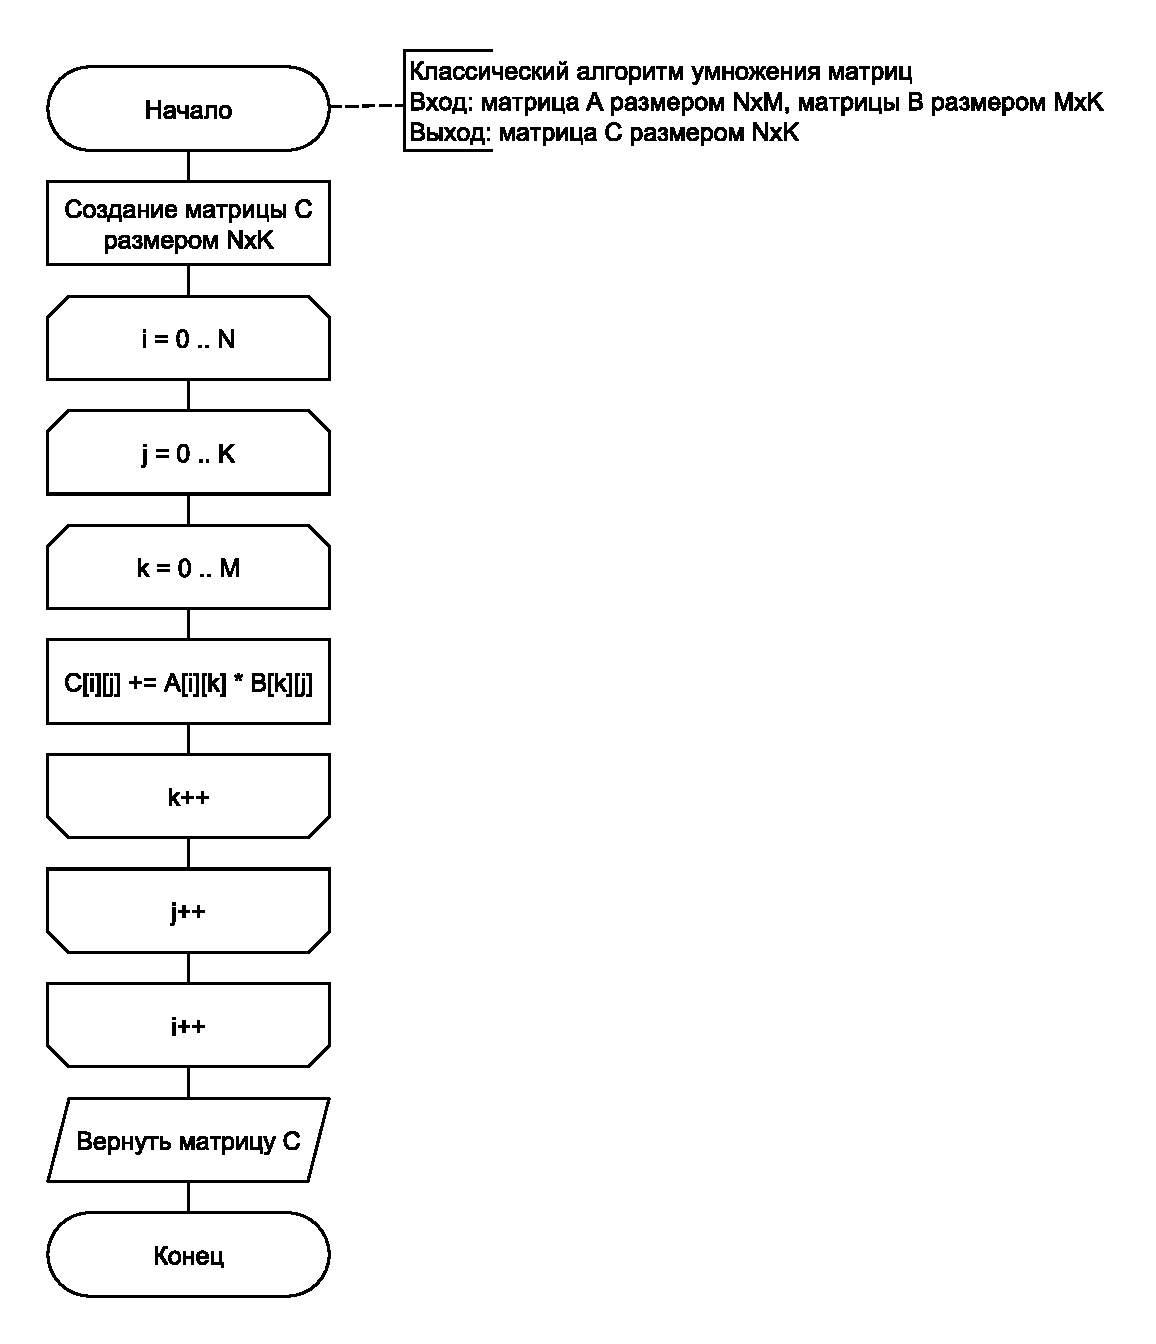
\includegraphics[]{img/default_mult.eps}
	\caption{Классический алгоритм умножения}
	\label{fig:def}
\end{figure}

\clearpage

\begin{figure}[h]
	\centering
	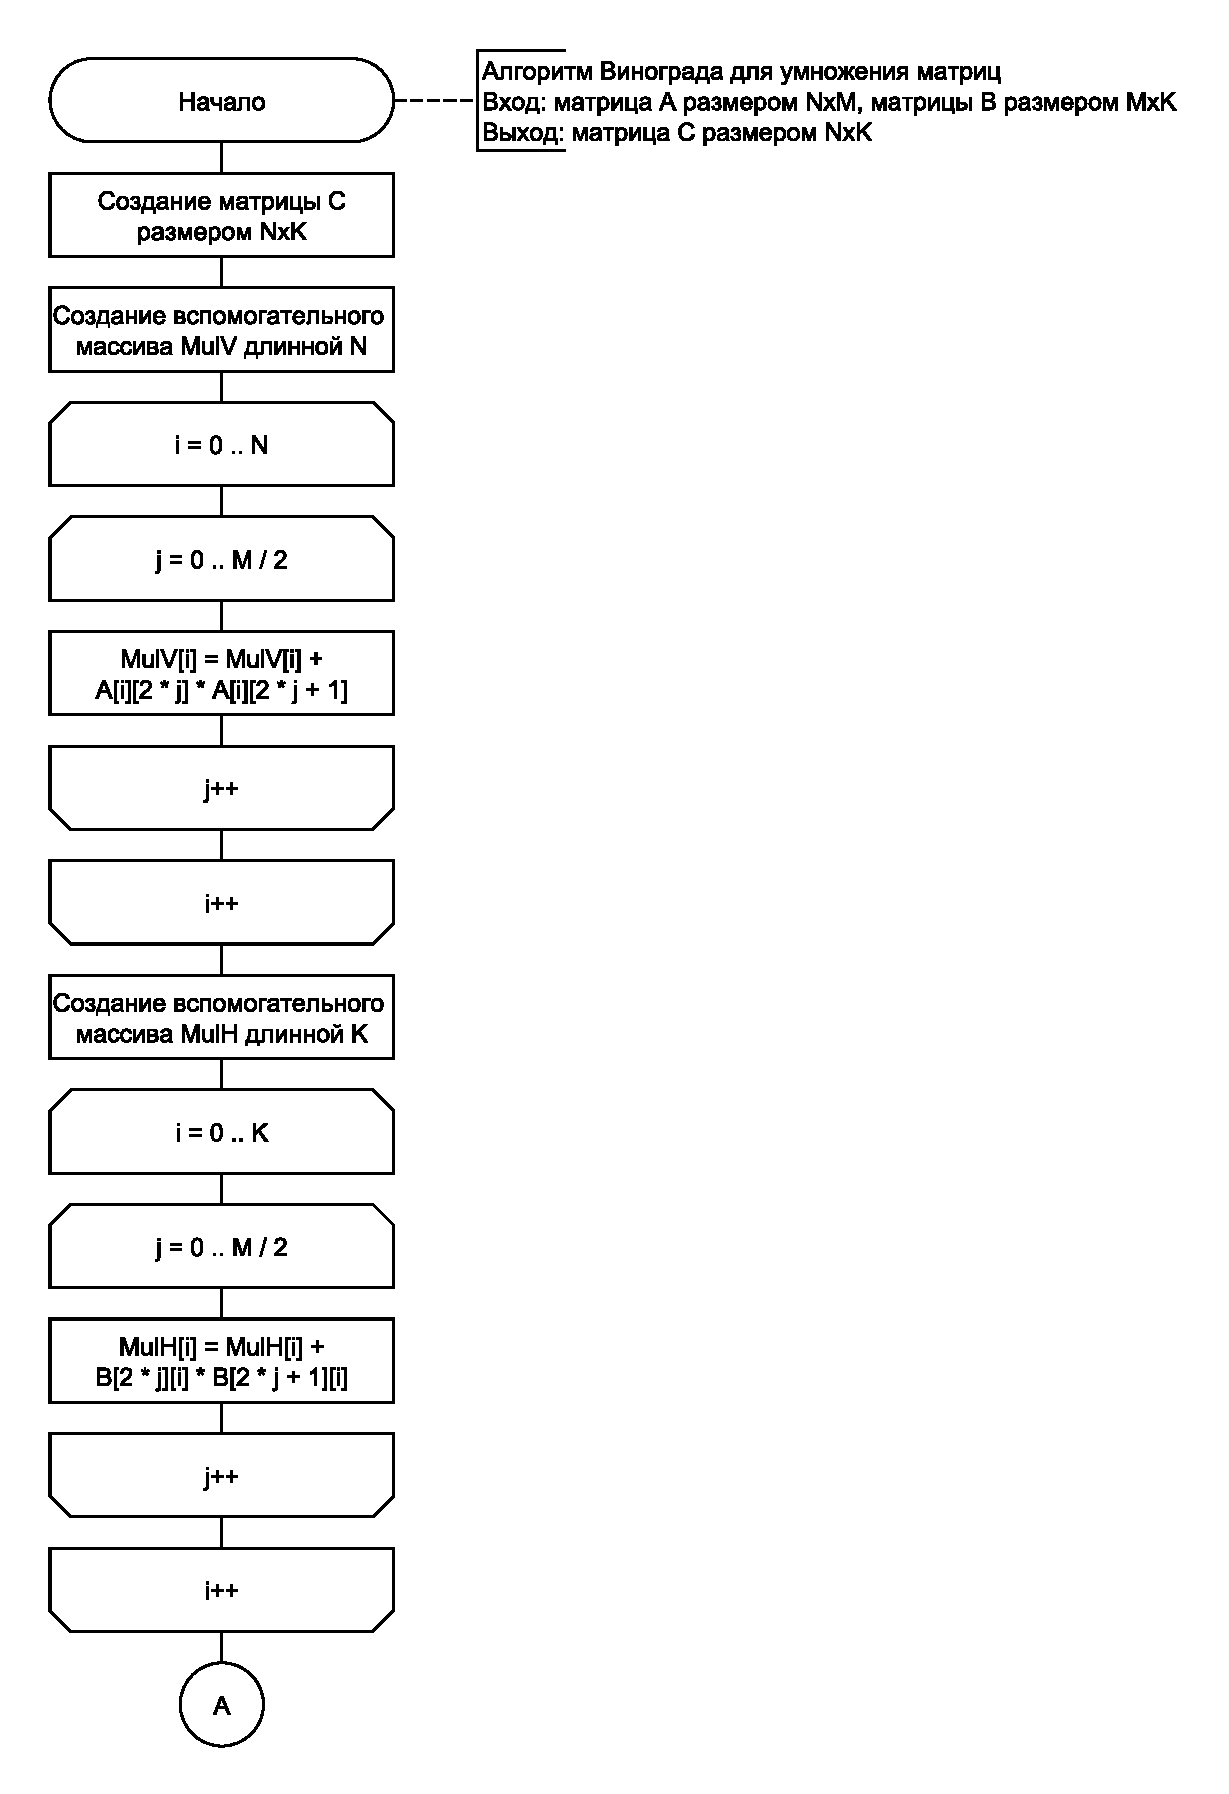
\includegraphics[scale=0.75]{img/vinograd_1.eps}
	\caption{Алгоритм Винограда, часть 1}
	\label{fig:vin1}
\end{figure}

\clearpage

\begin{figure}[h]
	\centering
	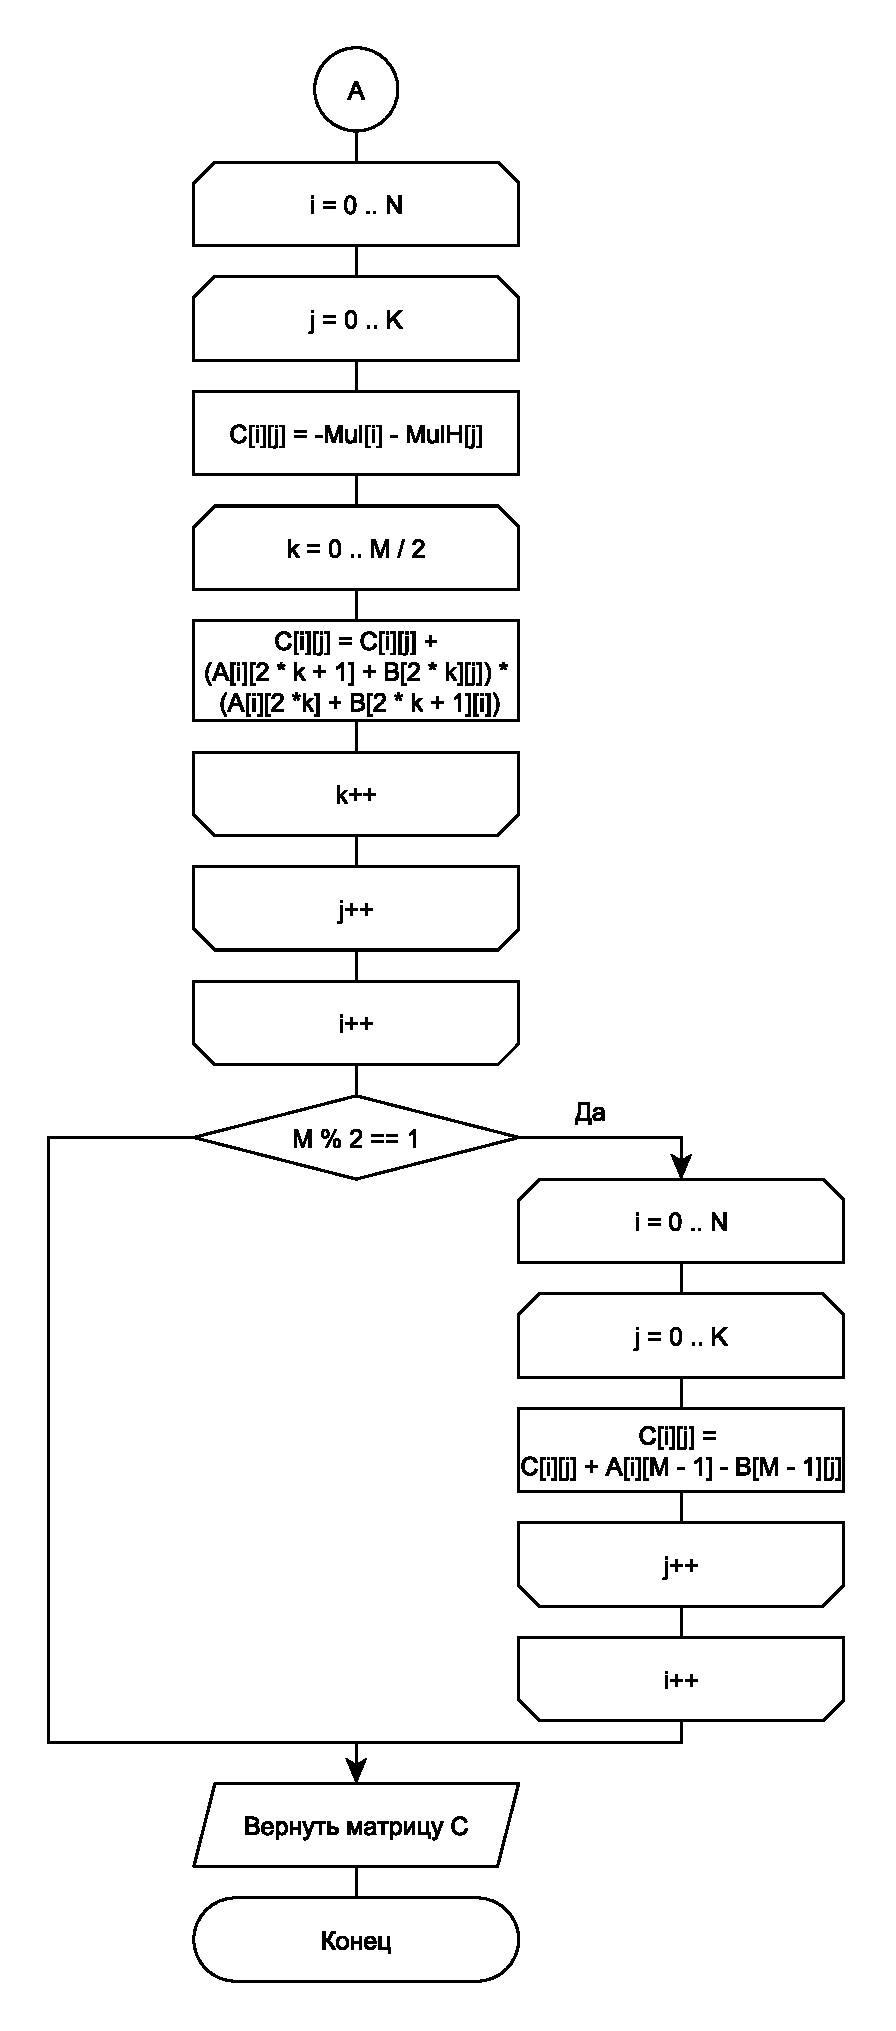
\includegraphics[scale=0.7]{img/vinograd_2.eps}
	\caption{Алгоритм Винограда, часть 2}
	\label{fig:vin2}
\end{figure}

\clearpage

\begin{figure}[h]
	\centering
	\includegraphics[scale=0.75]{img/vinograd_mod_1.eps}
	\caption{Модифицированный алгоритм Винограда, часть 1}
	\label{fig:mvin1}
\end{figure}

\clearpage

\begin{figure}[h]
	\centering
	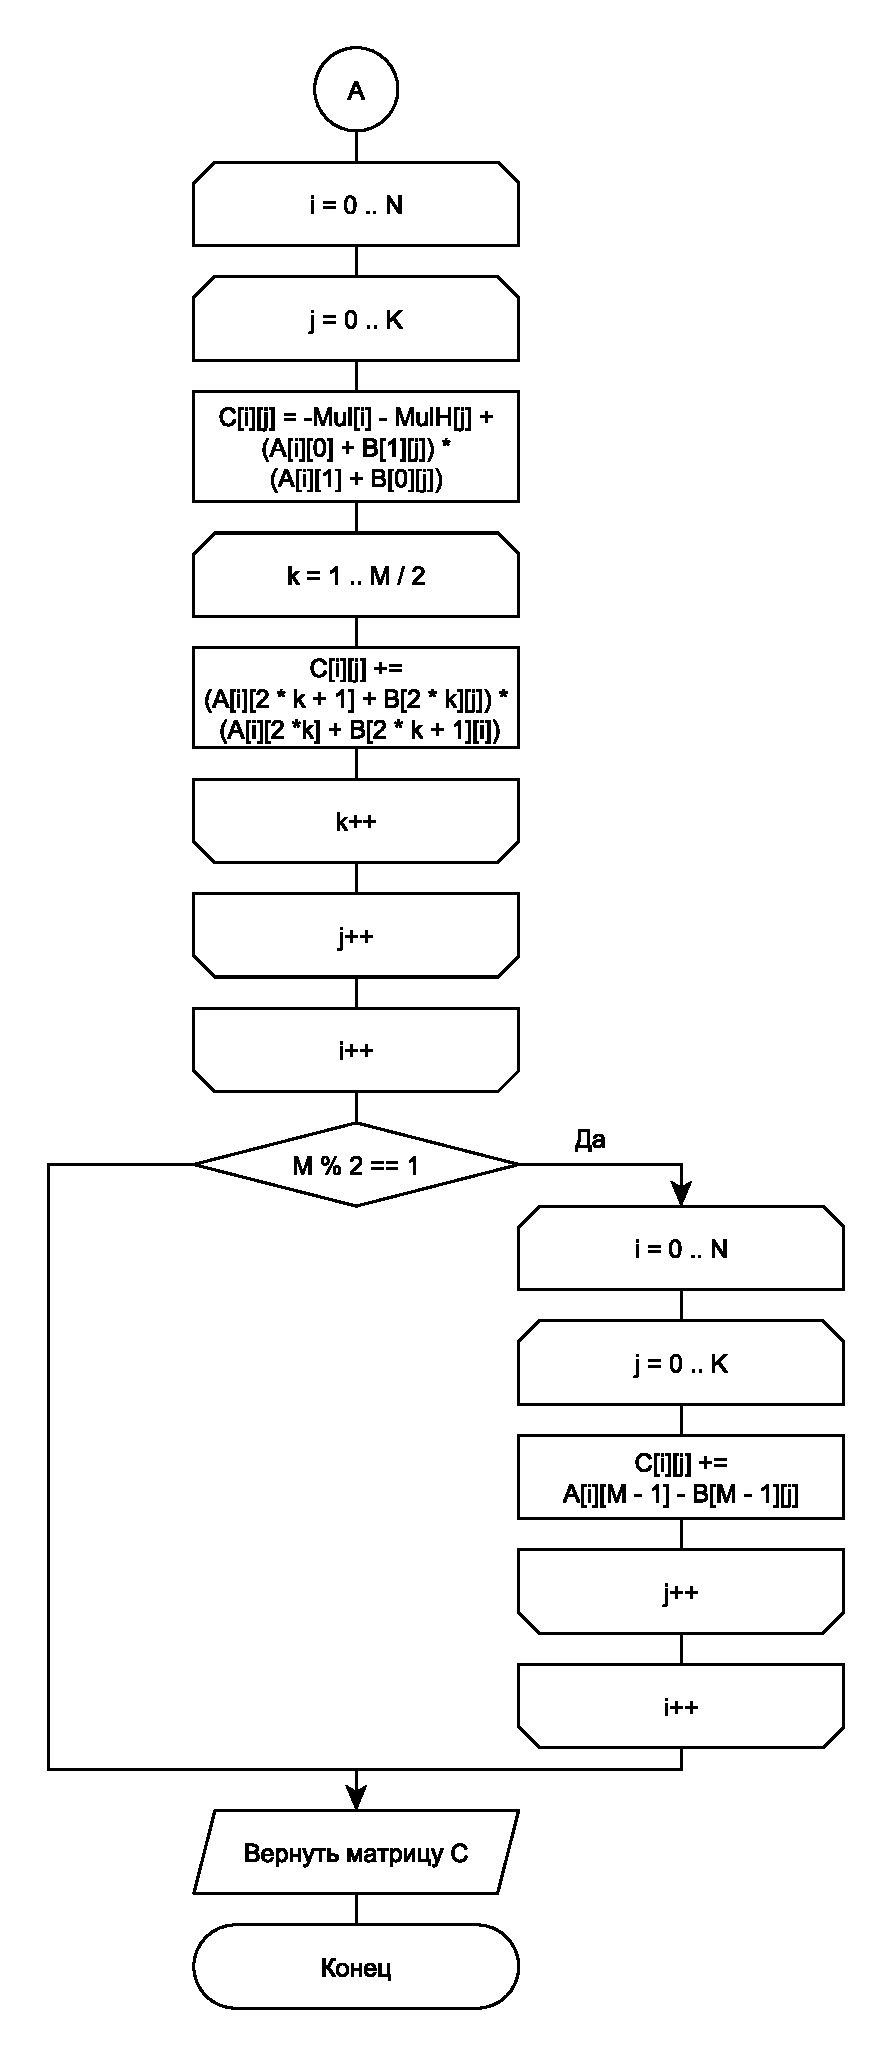
\includegraphics[scale=0.7]{img/vinograd_mod_2.eps}
	\caption{Модифицированный алгоритм Винограда, часть 2}
	\label{fig:mvin2}
\end{figure}

\clearpage

\section{Модель вычислений}
Для вычисления трудоемкости введем модель вычислений:
\begin{enumerate}
	\item операции из списка (\ref{for:opers}) имеют трудоемкость 1;
	\begin{equation}
		\label{for:opers}
		+, -, ==, !=, <, >, <=, >=, [], ++, {-}-
	\end{equation}
    \item операции из списка (\ref{for:opers_2}) имеют трудоемкость 2;
	\begin{equation}
		\label{for:opers_2}
		*, /, \%
	\end{equation}
	\item трудоемкость условного оператора \code{if условие then A else B} рассчитывается как (\ref{for:if});
	\begin{equation}
		\label{for:if}
		f_{if} = f_{\text{условия}} +
		\begin{cases}
			f_A, & \text{если условие выполняется,}\\
			f_B, & \text{иначе.}
		\end{cases}
	\end{equation}
	\item трудоемкость цикла рассчитывается как (\ref{for:for});
	\begin{equation}
		\label{for:for}
		f_{for} = f_{\text{инициализации}} + f_{\text{сравнения}} + N(f_{\text{тела}} + f_{\text{инкремента}} + f_{\text{сравнения}})
	\end{equation}
	\item трудоемкость вызова функции/возврата результата равна 0.
\end{enumerate}


\section{Трудоемкость алгоритмов}
% Перефразировать
В следующих частях будут рассчитаны трудоемкости представленных ранее классического алгоритма, алгоритма Винограда, оптимизированного алгоритма Винограда.
Трудоемкость инициализации результирующей матрицы учитываться не будет, поскольку данное действие есть во всех алгоритмах и не является самым трудоемким.

Введем обозначения:
\begin{itemize}
	\item[---] N --- количество строк первой матрицы;
	\item[---] M --- количество столбцов первой матрицы и количество строк второй матрицы;
	\item[---] K --- количество столбцов второй матрицы.
\end{itemize}

\subsection{Классический алгоритм умножения матриц}

Трудоемкость стандартного алгоритма умножения матриц состоит из:

\begin{itemize}
	\item[---] внешнего цикла по $i \in [1..N]$, трудоемкость которого: $f = 2 + N \cdot (2 + f_{body})$;
	\item[---] цикла по $j \in [1..K]$, трудоемкость которого: $f = 2 + K \cdot (2 + f_{body})$;
	\item[---] цикла по $k \in [1..M]$, трудоемкость которого: $f = 2 + 12 \cdot M$.
\end{itemize}

Трудоемкость классического алгоритма равна трудоемкости внешнего цикла.
Ее можно вычислить, подставив циклы тела (\ref{for:classic}):
\begin{equation}
	\label{for:classic}
	f_{classic} = 2 + N \cdot (4 + K \cdot (4 + 11M)) = 2 + 4N + 4NK + 14NMK \approx 14NMK
\end{equation}

\subsection{Алгоритм Винограда}

Трудоемкость алгоритма Винограда состоит из:
\begin{itemize}
	\item[---] создания и инициализации массивов MulV и MulH, трудоемкость которого (\ref{for:init}):
	\begin{equation}
		\label{for:init}
		f_{init} = N + K;
	\end{equation}
	
	\item[---] заполнения массива MulV, трудоемкость которого (\ref{for:MulV}):
	\begin{equation}
		\label{for:MulV}
		f_{MulV} = 2 + N \cdot (4 + \frac{M}{2} \cdot 19);
	\end{equation}
	
	\item[---] заполнения массива MulH, трудоемкость которого (\ref{for:MulH}):
	\begin{equation}
		\label{for:MulH}
		f_{MulH} = 2 + K \cdot (4 + \frac{M}{2} \cdot 19);
	\end{equation}
	
	\item[---] цикла заполнения для четных размеров, трудоемкость которого (\ref{for:cycle}):
	\begin{equation}
		\label{for:cycle}
		f_{cycle} = 2 + N \cdot (2 + K \cdot (2 + 7 + 4 + \frac{M}{2} \cdot (4 + 26)));		
	\end{equation}
	
	\item[---] цикла, для дополнения результирующего массива суммой последних нечетных строки и столбца, если общий размер нечетный, трудоемкость которого (\ref{for:last}):
	\begin{equation}
		\label{for:last}
		f_{last} = \begin{cases}
			2, & \text{размер четный,}\\
			2 + N \cdot (2 + 14K), & \text{иначе.}
		\end{cases}
	\end{equation}
\end{itemize}

Итого, результирующая трудоемкость алгоритма Винограда равна (\ref{for:final})
\begin{equation}
	\label{for:final}
	f_{final} = f_{init} + f_{MulV} + f_{MulH} + f_{cycle} + f_{last} \approx 15NMK
\end{equation}

Классический алгоритм Винограда имеет большую трудоемкость, чем классический алгоритм умножения матриц.

\subsection{Оптимизированный алгоритм Винограда}
Трудоемкость оптимизированного алгоритма Винограда состоит из:
\begin{itemize}
	\item[---] создания и инициализации массивов MulV и MulH а также доп. переменной, хранящей N/2, трудоемкость которого (\ref{for:init}):
	\begin{equation}
		\label{for:init}
		f_{init} = N + K;
	\end{equation}
	
	\item[---] заполнения массива MulV, трудоемкость которого (\ref{for:MulV}):
	\begin{equation}
		\label{for:MulV}
		f_{MulV} = 2 + N \cdot (4 + \frac{M}{2} \cdot 11);
	\end{equation}
	
	\item[---] заполнения массива MulH, трудоемкость которого (\ref{for:MulH}):
	\begin{equation}
		\label{for:MulH}
		f_{MulH} = 2 + K \cdot (4 + \frac{M}{2} \cdot 11);
	\end{equation}
	
	\item[---] цикла заполнения для четных размеров, трудоемкость которого (\ref{for:cycle}):
	\begin{equation}
		\label{for:cycle}
		f_{cycle} = 2 + N \cdot (2 + K \cdot (2 + 20 + 4 + (\frac{M}{2} - 1) \cdot (4 + 20)));
	\end{equation}
	\item[---] цикла, для дополнения результирующего массива суммой последних нечетных строки и столбца, если общий размер нечетный, трудоемкость которого (\ref{for:last}):
	\begin{equation}
		\label{for:last}
		f_{last} = \begin{cases}
			2, & \text{размер четный,}\\
			2 + N \cdot (2 + 11K), & \text{иначе.}
		\end{cases}
	\end{equation}
\end{itemize}

Итого, результирующая трудоемкость оптимизированного алгоритма Винограда равна (\ref{for:final})
\begin{equation}
	\label{for:final}
	f_{final} = f_{init} + f_{A1} + f_{B1} + f_{cycle} + f_{last} \approx 12NMK
\end{equation}

Оптимизированный алгоритм Винограда имеет меньшую трудоемкость, по сравнению с классическим алгоритмом.

\vspace{5mm}

\textbf{ВЫВОД}

В данном разделе были приведены схемы алгоритмов умножения матриц, а также были проведены расчеты трудоемкости каждого из трех алгоритмов.

\clearpage